In this section we model the problem as a bipartite graph matching problem. Then show that how it translates to the general case of online packing problem after some normalization.
\subsection{Graph Model}
Lets consider a bipartite graph $G = (V = \{L \cup R\}, E)$, where $V$ is the set of vertices; $L$ denotes the left partition of the vertices and $R$ the right partition. $E$ is the set of edges. We use such a bipartite to model our problem setting, where items are treated as nodes and edges denote a potential swap between two items. Consider the candidate item set $C$ is represented by the fixed vertex set $R$. The $L$ set is the set of all $r_{ij}$s, i.e. the set of all recommendations. The edge-weights represent the cost of the swap between $r_{ij}$ and $c$.\\
Recall in section~\ref{sec:pf}, the swap constraints imply that a candidate item cannot be swapped in more than once in a single item page, however can be swapped multiple times for different items. We model this by replicating the candidate set for every the item pages. This is shown in figure~\ref{fig:bipartite}. The figure depicts a simple scenario where there are only three items in the universe and one place to recommend item in each item page. Thus $|I| = 3$ and $k=1$. We are given one candidate item, $|C| = 1$. We replicate the candidate item thrice for each different item pages, as denoted by the vertices $R1, R2$ and $R3$ which results to the bipartite graph shown in figure~\ref{fig:bipartite}.\\
\begin{figure}[h]
  \centering
  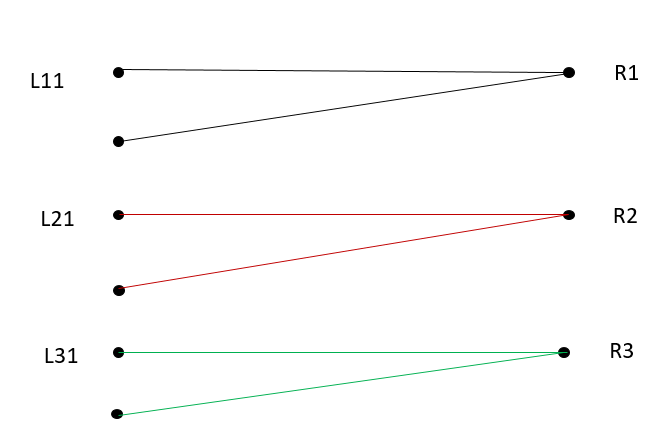
\includegraphics[width=3.3in]{figs/bipartite.png}
  \caption{Bipartite graph model}
  \label{fig:bipartite}
\end{figure}
In the online settings that we consider, however, we donot have the full graph given to us. At an time epoch $t$, we know a subset of $L$ nodes, representing the item subset being visited by some users. When such a node comes, its edges and the corresponding edge weights are revealed. Edge weights denote the cost of the swap at that epoch $t$. The rewards are the node weights. We treat the arrival of same item at different epoch as a different $L$ node. Thus at time epoch $t$, based on the $w$ vector a set of $L$ nodes and the corresponding edges are revealed. Thus figure~\ref{fig:bipartite} represents a snapshot of the graph at sometime $t$. \\
Given such bipartite graph the objective translates to the following linear equation.\\
\begin{equation}\label{eq:LP1}
\begin{split}
max \sum_{t \in T} \sum_{i = 1}^{|L|} \sum_{j = 1}^{|R|} w^t(i) \times x_{ij} \\
\text{such that} \\
\sum_{t \in T} \sum_{i = 1}^{|L|} \sum_{j = 1}^{|R|} c^t(i,j) \times x_{ij} \leq B \\
\sum_{i = 1}^{|L|} x_{ij} \leq 1 \\
\sum_{j = 1}^{|R|} x_{ij} \leq 1 \\
x_{ij} \in \{ 0,1 \}
\end{split}
\end{equation}
where $w^t(i)$ denotes the weight of node $i$ at time $t$ and $c^t(i,j)$ is the edge weight of edge $(i,j)$ at time $t$.
\subsection{Connection to multiple slot ad-allocation}
The multiple slot ad-allocation is a well studied combinatorial problem, where there are $m$ bidders, $n$ keywords and bid is done for $l$ slots. The $l$ slots to which ad-auctions can be allocated and suppose that buyers are
allowed to provide bids on keywords which are slot dependent. Denote the bid of buyer $i$ on keyword $j$ and
slot $k$ by $b(i, j, k)$. The restriction is that an (integral) allocation of a keyword to two different slots cannot be
sold to the same buyer. The linear programming formulation of the fractional version of the problem is shown in equation \ref{eq:LP2}.
\begin{equation}\label{eq:LP2}
\begin{split}
max \sum_{j=1}^m \sum_{i = 1}^{n} \sum_{l = 1}^{k} b(i,j,l) \times y(i,j,l) \\
\text{such that} \\
\sum_{j =1}^m \sum_{k = 1}^{l} b(i,j,k) \times y(i,j,k) \leq B(i) \\
\sum_{i = 1}^{n} y(i,j,k) \leq 1, \forall 1 \leq j \leq m, 1\leq k \leq l \\
\sum_{k = 1}^{l} y(i,j,k) \leq 1 , \forall 1 \leq j \leq m, 1 \leq i \leq n \\
\end{split}
\end{equation}
\ \\
Clearly this is very similar to our problem of equation \ref{eq:LP1}. Buchbinder et al in \cite{buchbinder2007online} has proposed an elegant algorithm for the online version of the problem. We extend that in section \ref{sec:alg2} to solve our problem.
\subsection{Reducing to online packing}
We now reduce the equation~\ref{eq:LP1} to the general form of online packing problem. The general form of online packing (dual) and the corresponding primal, which is also called covering is shown in figure~\ref{fig:pd}.\\
\begin{figure}[h]
  \centering
  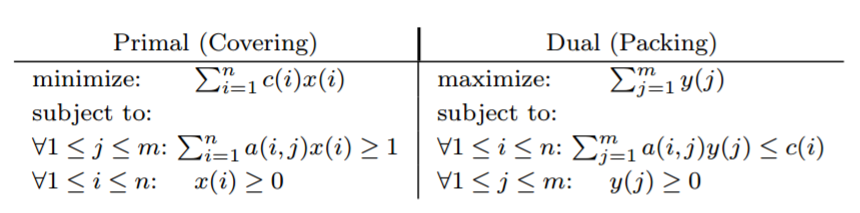
\includegraphics[width=3.3in]{figs/primal-dual.png}
  \caption{Primal (covering) and dual (packing) problem}
  \label{fig:pd}
\end{figure}
The transformation steps are as follows:
\begin{itemize}
\item Normalize the edge weights with the corresponding node weight of the left node to which they are incident to. This get rids of the $w(i)$s and $a(i,j) = c(i,j) / w(i)$.
\item We relax the $x_{ij} \in \{0,1\}$ to $x_{ij} \geq 0$. This corresponds to fractional matching, which is unrealistic in our settings. However we show that we can use randomized rounding that preserves feasibility with $O(1)$ loss inn objective.
\item Finally we normalize the $a(i,j)$ such that, $a(i,j) \in [0,1]$. For that we assume a high enough $a^\ast(i,j)$, so that $a^\ast(i,j)$ is greater than any $a(i,j)$. Then set $a(i,j) = a(i,j) /a^\ast(i,j) $. The budget is also scaled down as $b = B /a^\ast(i,j) $.
\end{itemize}
As in the online setting, we donot know the $a(i,j)$s in advance. They are revealed with arrival of each $y(j)$ and decision to include $y(j)$ in packing is irrevocable.\\
Note that the third step of the transformation requires the prior knowledge on the bound of the edge weights. This may not always be available. Thus in section~\ref{sec:alg}, we present two different schemes, one that does not require $a^\ast(i,j)$ to be known. This schemes violates the budget constraints, although we show that the violation is not too much (will be formalized). The second schemes assumes known $a^\ast(i,j)$, and uses that to produce perfectly feasible solution. The randomized rounding is used inn both schemes with $O(1)$ loss in objective. 
